\chapter{Ist-Analyse ( 5 \%)}
\label{chap:ist-analyse}

Dieses Kapitel dient der Beschreibung existierender System.
Es soll ihre Eigenschaften und Probleme aufzeigen.
Diese werden zuerst Theoretisch betrachtet und
dann an Systemen in der Praxis demonstriert.

% dieses kap dient .. und damit soll .. aufbau

\section{Eigenschaften der existierenden Systeme}

\subsection{Struktur}
\label{sec:ist-analyse:struktur}

Wie in der folgenden Grafik leicht zu erkennen,
sind traditionellen CI-Systeme Client-Server Systeme.

\begin{figure}[ht]
  \centering
  \label{fig:ist-aufbau-tradition}
  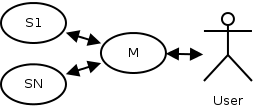
\includegraphics[height=1in]{imageinput/ist-aufbau-tradition.png}
  \caption{Logischer Aufbau eines CI System}
\end{figure}

Der sogenannte Master ist der Server und verwaltet alle Daten.
Die Slaves sind die Clients und verrichten die eigentliche Arbeit.
Sie sammeln Daten und liefern diese einschliesslich der Resultate beim Master ab.

Benutzer interagieren Ausschliesslich mit dem Master.

\subsection{Datensammlung}
Wie bereits in Sektion~\ref{sec:base:ci} erw\"ahnt,
f\"uhrt ein CI-System nicht nur Auftr\"age aus,
sondern sammelt auch daten f\"ur die sp\"atere Weiterverarbeitung.

Die Datensammlung l\"asst sich dabei grob in 2 Bereiche einteilen.
Zum einen die Laufzeitdaten und zum anderen die Artefakte.

Laufeitdaten fallen bereits w\"ahrend der Ausf\"uhrung an,
und beinhalten in der Regel zumindest die Textuellen Ausgaben
der ausgef\"uhrten Programme.
Weitere M\"oglichkeiten k\"onnen Testresultate, echzeit Logs und Ausf\"uhrungsstatistiken sein.
Laufzeitdaten werden dem Benutzer in idr. Zeitnah zur Verf\"ugung gestellt.

Artefakte hingegen sind Dateien,
welche erst nach Abschluss eines Schrittes zur verf\"ugung stehen.
Zu ihnen gehoeren neben den traditionellen ausf\"uhrbaren Dateien
auch lauff\"ahige Archive des Gesammtprogrammes oder Testergebnisse in den Formaten JunitXML oder TAP.

%XXX: cite tap, junitxml

Diese werden zum Master geschickt, dort aufbewahrt und sp\"ater genutzt.

In der Regel werden ausf\"uhrbare Artefakte zum Download angeboten,
w\"ahrend Testergebnisse nur dargestellt werden.





\section{Probleme existierender Systeme}

Diese Sektion gibt einen \"Uberblick \"uber die Problemarten existierender Ststeme

\subsection{Datenzugriff}

Beim Datenzugriff sind die existierenden Systeme besonders Problematisch.
Es gibt Grunds\"atzlich keinerlei Standardschnittstellen.
Die meisten Systeme verwenden noch nicht einmal eine Datenbank.
Jene welche doch eine verwenden wird, machen sie nicht zug\"anglich.

Die Datenhaltung dieser Systeme kann somit grob als geordnete Ablage klassifiziert werden. Weiterf\"uhrende Abfragen sind nicht m\"oglich.

\subsection{Erweiterbarkeit}

Die Erweiterbarkeit eines CI-Systemes wird von 2 Hauptpunkten dominiert.
Dies ist die Integration in die Benutzeroberfl\"ache
und zum anderen die M\"oglichkeiten mit den Daten interagieren
und auf neue Weise zu kombinieren.

Die erweiterbaren Systeme stellen normalerweise zumindest eine Schnittstelle
f\"ur die graphische Oberfl\"ache zur Verf\"ugung.
Damit ist zumindest das problemlose Anpassen der Benutzerschnittstelle gegeben.


F\"ur eigene Analysewerkzeuge kann es jedoch oft notwendig werden,
eine eigene Datenbank, welche vom CI-System getrennt ist zu verwenden.
Einige Anbieter von CI-werkzeugen w\"unschen dies sogar explizit.
%XXX:


\subsection{Komponentenabh\"angigkeit}

Wie bereits in Kapitel~\ref{sec:ist-analyse:struktur} erw\"ahnt,
sind CI-Systeme in der Regel traditionelle Netzwerksysteme die nach dem Client/Server Prinzip operieren.
Dabei sind die Rollen strikt als Master und Slave eingeteilt und das Management wird zentral im Master vorgenommen.
Slaves haben dabei keinerlei Autonomie und folgen strikt den Anweisungen des Master.

Dadurch nimmt das System zwar keinen Schaden wenn ein Slave ausf\"allt,
der Ausfall des Master ist jedoch fatal und kann nicht abgefangen werden.
Die stellt einen ``Single Point of Failure'' dar.


\section{Praxisbeispiele}

Um Probleme in der Praxis aufzuzeigen,
soll eine Auswahl and Werzeugen getroffen werden.
Anschliessend sollen ihre Eigenschaften und Probleme
n\"aher untersucht werden.


\subsection{Auswahl}

Um die Analyse von Praxisbeispielen zu erm\"oglichen,
sollen Systeme mit gewissen Rahmenbedingungen ausgew\"ahlt werden.
Wichtigs Kritierum ist dabei, das sie \textbf{open-source} Software sind,
oder zumindest \"offentlich verf\"ugbar sind.
Sie sollten \textbf{verbreitet} sein, damit ein \"Uberblick
\"uber praxisrelevante Probleme geschaffen.
Ausserdem sollten sie \textit{kostenlos} sein,
%XXX> LOL
\textit{um den finanziellen Ruin eines hilflosen Studenten zu verhindern}.

Ausgew\"ahlt wurden die Systeme
\begin{itemize}
  \item Jenkins/Hudson
  \item Buildbot
  \item TravisCI
\end{itemize}


\subsection{Jenkins/Hudson}

Jenkins und Hudson sind aus der Java Welt  stammende CI-Systeme.
Sie bieten alle Grundfunktionen, um grundlegendes CI umzusetzen
und unterst\"utzen auch erweiterte Funktionen,
wie Matriz-Build und nachgelagerte Builds.

Sie stellen ein einfach zu bedienendes Nutzerinterface zur verf\"ugung,
Konfiguration findet jedoch nur im Rahmen dieses Interfaces statt.

Erweiterte Parametrisierung ist nicht m\"oglich.
Auch Entwicklungszweige sind dem System unbekannt,
m\"ochte man mehr als einen dem Testprozess unterziehen,
so muss ein weiterer Job angelegt werden.

Zugriff auf die Daten kann nur mittels der internen API oder
einer nicht dokumentierten REST API genommen werden.

Damit war es nicht m\"oglich in annehmbarer Zeit festzustellen,
in wie weit sich die UseCases umsetzen lassen.
Das System verwendet Augenscheinlich kein DBMS.
Datenabfragen und Aggregationen m\"ussen
somit von Hand ausformuliert werden.

Das Konzept der Build-Artefakte wird unterst\"utzt und
aktiv f\"ur Funktionen wie nachgelagerte Builds verwendet.

Es gibt einige simplel gestrickte Plugins mit dem Zweck testresultate anzuzeigen,
jedoch wird auf weitergehende Analysen dieser Resultate g\"anzlich verzichtet
Mehr als eine Historie gibt es nicht.


\subsection{Buildbot}


BuildBot positioniert sich als eine Art Meta-Build-Server.
Es biete keine normale Benutzerschnittstelle zur Konfiguration,
sondern wird mittels Komposition von Metadaten und Komponenten konfiguriert.

Die Konfiguration des Servers stellt dabei ein Pythons-Script,
welches die gewünschten Jobs zusammenstellt und den Server konfiguriert.
Matrix-Builds werden nicht unterst\"utzt,
k\"onnen aber in Teilen durch das verwenden von Schleifen im Script simuliert werden.
Es ist möglich Builds Jobs mit minimale Parameter in Form von Strings zu Übergeben,
dabei kann man auch den Entwicklungszweig mit angeben.

Builbot unterst\"utzt das Sammeln von Daten in sog. Logdateien,
diese sind intern ind extern leicht Auffindbar.
Es gibt sogar schon Werkzeuge, welche dies zur erweiterten Vergleichen von Testresultaten nutzen nutzen.

%XXX referenzen
%XXX: C
Einige wurden dabei besonders genau betrachtet.
Das erste ist der PYPY Buildbot, welcher eine hilfreiche Gesammt\"ubersicht der Testfehler
der letzten 4 Builds darstellt.
Das zweite ist das Script names ``compare\_last\_builds.py'' aus dem PYPY Projekt,
welches die Unterschiede in den Testresultaten zwischen 2 Builds hervorhebt.
Sie werden sp\"ater als Ideenlieferant dienen.

Tragisch ist, das die Buildbot entwickler selbst,
es nicht als Aufgabe ihres Systemes sehen, sich mit Testergebnissen zu befassen,
sie empfehlen Integration externer Komponenten.

\subsection{TravisCI}


%XXX refs
TravisCI ist wesentlich anders Positioniert, als die beiden voehergehenden Systeme.
Es setzt zusammenarbeit in den vordergrund und der Breiten masse werden Server zur verf\"ugung gestellt.
Diese behandlen die Integration von Projjekten, welche auf der beliebten Code-Hosting Site GitHub gemanagt werden.
% ref yaml
Die Konfiguration ist dabei Zweigeteilt,
eine Datei im YAML Format legt dabei Build-Achsen und Schritte fest.
Diese Datei befindet sich in Versionskontrolle beim Projekt
(was die Konfiguration sehr Flexibel gestaltet)

Ist ein Projekt erst einmal im System registriert,
so wird es regelmaessig bei \"anderungen Integriert.

Besonders hilfreich ist dabei, das TravisCI auch den fall behandelt, wenn ein anderer Benutzer der Code-Hosting Seite a\"nderungen anmeldet.
Die Testet es auch, und Markiert sogar das Resultat.

Was leider nichts daran \"andert, das TravisCI keine externe API zur verf\"ugung stellt.
Es ist ein geschlossenes System. Auch hat es absolut kein Konzept f\"ur Datensammlung/Artefakte.
Es ist nicht portabel und scheinbar f\"ur den Betrieb nur auf den zur verf\"ugung gestellten Servern vorgesehen.


\section{Zusammenfassung}

Dieses Kapitel hat die Probleme der CI-Systeme n\"aher gezeigt.
Wir haben gesehen, dass Datenzugriff und Erweiterungen f\"ur Analyse,
schwer oder gar nicht zu erreichen sind.
Ausserdem sind die Systeme nach einegen Klassen nicht direkt wiederherstellbar.
Im Folgenden Verlauf der Arbeit soll der Grundstein f\"ur ein CI-System gelegt werden,
Welches Datanzugriff und Datenanalyse vereinfacht.
Zus\"atzlich soll es Gunds\"atzliche fehlertolleranz aufweisen.


